\documentclass{math}

\usepackage{tikz}

\title{University Physics 1A}
\author{Alvin Lin}
\date{November 6th, 2017}

\begin{document}

\maketitle

\section*{Torque}
To calculate the acceleration of an object rolling down a ramp.
\begin{center}
  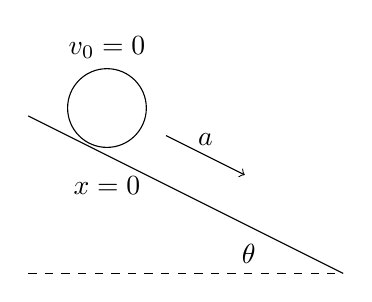
\begin{tikzpicture}
    \draw (-2,2) -- (2,0);
    \draw (-1,2.1) circle (0.5cm) node[below,yshift=-0.75cm] {\( x = 0 \)}
      node[above,yshift=0.5cm] {\( v_0 = 0 \)};
    \draw[->] (-0.25,1.75) -- (0.75,1.25) node[pos=0.5,above] {\( a \)};
    \draw[dashed] (-2,0) -- (2,0) node[pos=0.7,above] {\( \theta \)};
  \end{tikzpicture}
\end{center}
\begin{align*}
  N-mg\cos\theta &= 0 \\
  mg\sin\theta-f &= ma \\
  fr &= \tau = I\alpha \\
  a &= r\alpha \\
  &= r\frac{fr}{I} \\
  &= \frac{r^2}{I}(mg\sin\theta-ma) \\
  a(1+\frac{mr^2}{I}) &= \frac{r^2mg\sin\theta}{I} \\
  a &= \frac{r^2mg\sin\theta}{I}\frac{1}{(1+\frac{mr^2}{I})} \\
  &= \frac{r^2mg\sin\theta}{I+mr^2} \\
\end{align*}
Using Conservation of Energy:
\begin{align*}
  mgh &= \frac{1}{2}mv^2+\frac{1}{2}I\omega^2 \\
  mgh &= \frac{1}{2}mv^2+\frac{1}{2}I\frac{v^2}{r^2} \\
  mgh &= \left(\frac{1}{2}m+\frac{I}{2r^2}\right)v^2 \\
  gh &= \frac{1}{2}(1+\frac{I}{mr^2})v^2 \\
  v^2 &= \frac{2gh}{1+\frac{I}{mr^2}}
\end{align*}
Plugging into the kinematic equations:
\begin{align*}
  v_f^2 &= v_i^2+2a(\Delta x) \\
  \frac{2gh}{1+\frac{I}{mr^2}} &= 2a\frac{h}{\sin\theta} \\
  a &= \frac{g\sin\theta}{1+\frac{I}{mr^2}} \\
  &= \frac{mg\sin\theta}{m+\frac{I}{r^2}}
\end{align*}

\subsection*{Experiment}
\begin{center}
  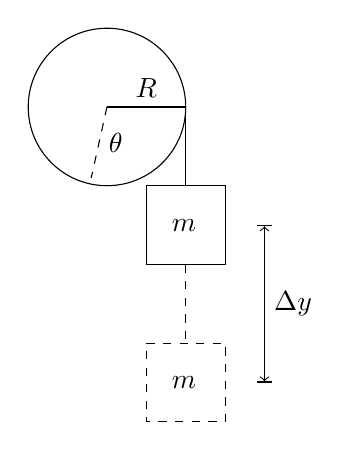
\begin{tikzpicture}
    \draw (0,0) circle (1cm);
    \draw (0,0) -- (1,0) node[pos=0.5,above] {\( R \)};
    \draw[dashed] (0,0) -- (-0.2,-0.9) node[pos=0.5,right] {\( \theta \)};
    \draw (1,0) -- (1,-1);
    \draw (0.5,-1) -- (1.5,-1) -- (1.5,-2) -- (0.5,-2) -- cycle
      node[pos=0.5,right,xshift=0.2cm] {\( m \)};
    \draw[dashed] (1,-2) -- (1,-3);
    \draw[dashed] (0.5,-3) -- (1.5,-3) -- (1.5,-4) -- (0.5,-4) -- cycle
      node[pos=0.5,right,xshift=0.2cm] {\( m \)};
    \draw[|<->|] (2,-1.5) -- (2,-3.5) node[pos=0.5,right] {\( \Delta y \)};
  \end{tikzpicture}
\end{center}
Find a formula for \( I \) in terms of \( \alpha \).
\begin{align*}
  \Delta y &= s = R\theta \\
  -\frac{I\alpha}{R}-mg &= ma \\
  &= mR\alpha \\
  -\frac{I\alpha}{R}-mR\alpha &= mg \\
  -\frac{I\alpha}{R} &= mg+mR\alpha \\
  I &= -\frac{R}{\alpha}(mg+mR\alpha) \\
  &= -\frac{mgR}{\alpha}-mR^2
\end{align*}

\begin{center}
  You can find all my notes at \url{http://omgimanerd.tech/notes}. If you have
  any questions, comments, or concerns, please contact me at
  alvin@omgimanerd.tech
\end{center}

\end{document}
